\subsection{LDR (light dependent resistor)} % (fold)
\label{sub:LDR_(light_dependent_resistor}
\begin{frame}
    \frametitle{LDR}
    \framesubtitle{}
     \begin{columns}[c]
        \column{0.6\textwidth}
            \begin{block}{Aufgabenstellung}
                 \begin{itemize}
                     \item Widerstandsmessung bei Verdunkeln
                     \item Dämmerungsschaltung
                 \end{itemize}
            \end{block}
        \column{0.4\textwidth}
            \begin{figure}[H]
            \begin{center}
                    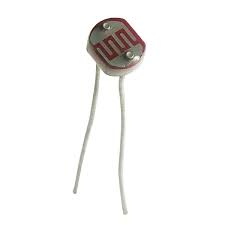
\includegraphics[scale=0.2]{./img/misc/ldr.jpeg}
            \end{center}
            \end{figure}
     \end{columns}
\end{frame}
\begin{frame}
    \frametitle{Verdunkeln}
    \framesubtitle{}
        \begin{tabular}{c|c|c}
        & $R/k\Omega$ & $\text{Lichstärke}/Lux$ \\
        \hline
        normale Beleuchtung & 0.34& $\approx 1000$  \\
        Verdunkeln & 70&$\approx 0.5$ \\
        \end{tabular}  
        \begin{block}{}
            \begin{itemize}
                \item LDR erhöht Widerstand bei Abdunkelung
            \end{itemize}
                \item Sehr hohe Widerstände bei starker Verdunkelung $R \approx
                2.5M\Omega$ beobachtet
        \end{block}
\end{frame}
\begin{frame}
    \frametitle{Dämmerungsschaltung}
    \framesubtitle{}
     \begin{columns}[c]
         \column{0.6\textwidth}
            \begin{block}{Wann leuchtet LED in der Nacht?}
                 \begin{itemize}
                     \item Spannungsabfall an Transistor (über $R_{pot} +
                     1k\Omega$) $U_{BE} \geq 0.58V$ um Transistor zu schalten
                     \begin{gather*}
                         \frac{U_{BE}}{U_{LDR}}=\frac{R_{Pot}+1k\Omega}{R_{LDR}} \\
                         R_{pot}
                         =
                         \frac{U_{BE}}{U_{LDR}} \cdot R_{LDR} - 1k\Omega \\
                         =
                         \frac{0.58V}{8.42V} 70k\Omega - 1k\Omega
                         \geq
                         3.8k\Omega
                     \end{gather*}
                 \end{itemize}
            \end{block}
         \column{0.4\textwidth}
             \begin{figure}[H]
             \begin{center}
                     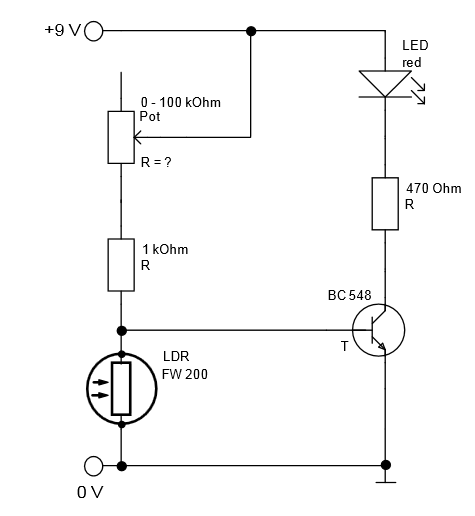
\includegraphics[scale=0.4]{./img/schaltung/ldr_2.png}
             \end{center}
             \end{figure}
     \end{columns}
\end{frame}
\begin{frame}
    \frametitle{Dämmerungsschaltung}
    \framesubtitle{}
    \begin{columns}[c]
        \column{0.6\textwidth}
            \begin{block}{Funktionsweise}
            \begin{itemize}
                \item LED leuchtet wenn
                \begin{equation*}
                    R_{pot} \geq \frac{0.58k\Omega}{8.42k\Omega} \cdot R_{LDR} -1k\Omega$ 
                \end{equation*}
                \item $\rightarrow$ je höher $R_{pot}$, desto insensitiver ist
                die Schaltung (höhere Variabilität bei $R_{LDR}$)
            \end{itemize}     
            \end{block}
        \column{0.4\textwidth}
            \begin{figure}[H]
            \begin{center}
                    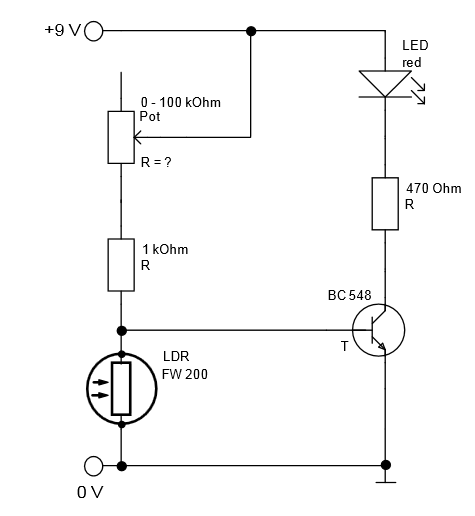
\includegraphics[scale=0.4]{./img/schaltung/ldr_2.png}
            \end{center}
            \end{figure}
    \end{columns}
\end{frame}


% subsection LDR (light dependent rcesistor (end)
